\chapter{Rectangular Waveguide(3)}
%\begin{figure}
%	\centering
%	\includegraphics[width=1\linewidth]{Schematic-of-a-rectangular-waveguide-extending-along-z-a-and-the-TE10-top-and-TE11}
%	\caption{}
%	\label{fig:schematic-of-a-rectangular-waveguide-extending-along-z-a-and-the-te10-top-and-te11}
%\end{figure}
In the previous lecture we try to visualize electric field inside a parallel plane waveguide. We also investigated the modal characteristics of a rectangular waveguide. We found that the modes which first propagate on a rectangular waveguide is a transverse electric mode with index (1, 0). We call that the DOMINANT MODE OF RECTANGULAR WAVEGUIDE. 
	
We also argue that most of the time we went on to operate in this single mode or dominant mode on the waveguide to avoid dispersion i.e broadening of the signal in time domain and as it travels on a guided structure. So this $TE_{10}$  is the most important mode for a rectangular waveguide, because most of the times, the energy is going propagate in this mode. So when this conduct experiments in the laboratory or we go to the fields, most of the time we deal with dominant mode,  $TE_{10}$ mode.


In this lecture we shall see the modal properties of the $TE_{10}$, mode and visualize the fields for $TE_{10}$ mode and then go to  calculation of what is called attenuation constant of  a waveguide. Because whenever we have a particular structure, we never have an
ideal dielectric in practice or ideal conductors. As a result there is always a loss in the walls of waveguides and also losses in the medium which is filling the waveguides.
So after visualizing the fields for $TE_{10}$ mode, in the waveguide, then we go to the calculation of attenuation constant in the rectangular waveguides.

We recall that for the rectangular waveguide,
\begin{equation}
E_{x} = E_{z} = H_{y} = 0
\end{equation}	
\begin{equation}
E_{y} = \dfrac{-j\omega\mu a }{\pi} C\sin \dfrac{\pi a}{x} e ^{-j\beta z}
\end{equation}
\begin{equation}
H_{x} = \dfrac{-j\omega a}{\pi} C \sin\dfrac{\pi a}{x}
	e^{-j\beta z} 
\end{equation}
\begin{equation}
H_{z} = C\cos \dfrac{\pi x}{a} e^{-j\beta z}
\end{equation}
There was no Y component for magnetic field. There was no Z component for electric field. We tried to visualize the fields for parallel plane waveguide, we get something like 
\begin{equation}
Re[E_{y}] = A\sin\dfrac{\pi x}{a} \sin\dfrac{2\pi}{\lambda g}z
\end{equation}	
\begin{equation}
Re[H_{x}] = B\sin\dfrac{\pi x}{a} \sin\dfrac{2\pi}{\lambda g}z
\end{equation}
\begin{equation}
Re[H_{z}] = C\cos\dfrac{\pi x}{a} \cos\dfrac{2\pi}{\lambda g}z
\end{equation}
Essentially this were the fields we visualized inside a
parallel plane waveguide.
\begin{equation}
Re[E_{y}] = A\sin\dfrac{\pi x}{a} \cos\dfrac{2\pi}{\lambda g}z
\end{equation}
if Z = 0, $E_{y}$ is zero. At a distance $ Z = \frac{\lambda g}{4}$, $E_{y}$ is maximum for variation in Z.

If we move the origin such that $Z = \frac{\lambda g}{4}$ is now the starting point shown.
\begin{figure}[h]
\centering
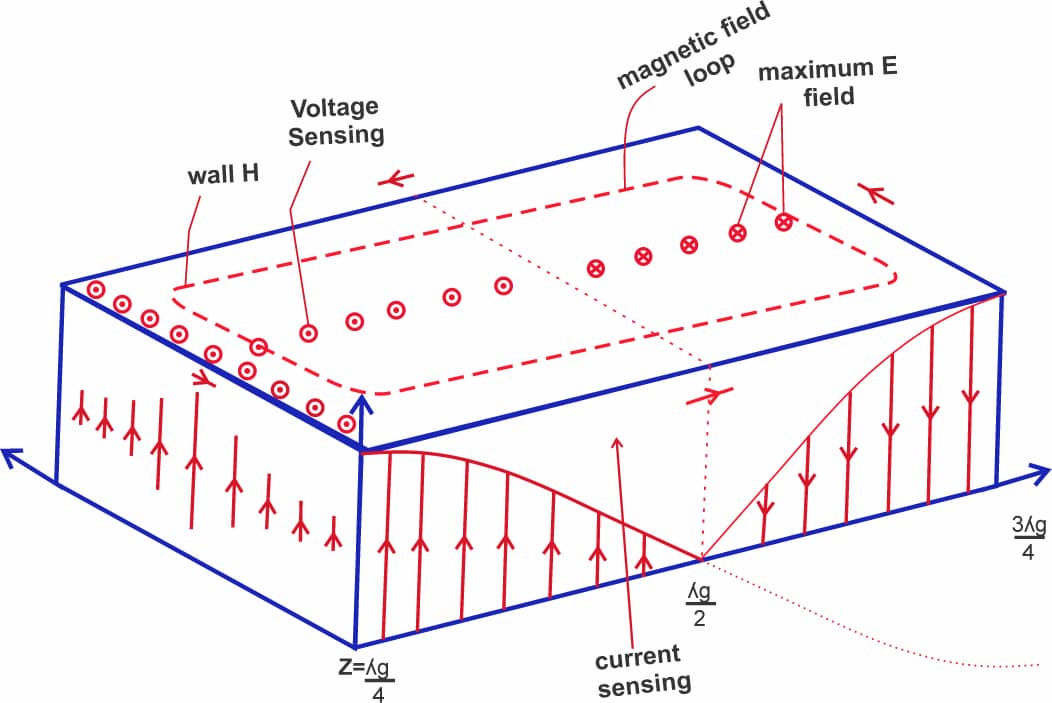
\includegraphics[width=1\linewidth]{./graphics/lecture-image-2.jpg}
\caption{EM WAVE OF A RECTANGULAR WAVE GUIDE SHOWING THE DIFFERENT FIELD}
\end{figure}
$E_{y}$ will have maximum value at   with sinusoidal variation along x as shown by the length of arrows and they all point in the positive y direction for $x = 0$ to $x = a$. Looking from the top, we have the variation shown with $\odot$ and $\otimes$ showing direction of the field looking from top.
 
The size of the circles shows the strength of the field. So if we go side ways the field has sinusoidal decrease, till it gets to zero at the edges.
 
As we move in the z directions, $E_{y}$ has sinusoidal variation in the z direction and the fields are shown in similar manner. Looking from the side we see the illustration corresponding to sinusoidal variation of the fields as shown. 
So we can write down the plane and the side view for the waveguide.
Visualizing the electric field is very simple as we visualize one component of the electric field which is Y oriented. Same thing we can do for the magnetic fields.
\begin{figure}[h]
\centering
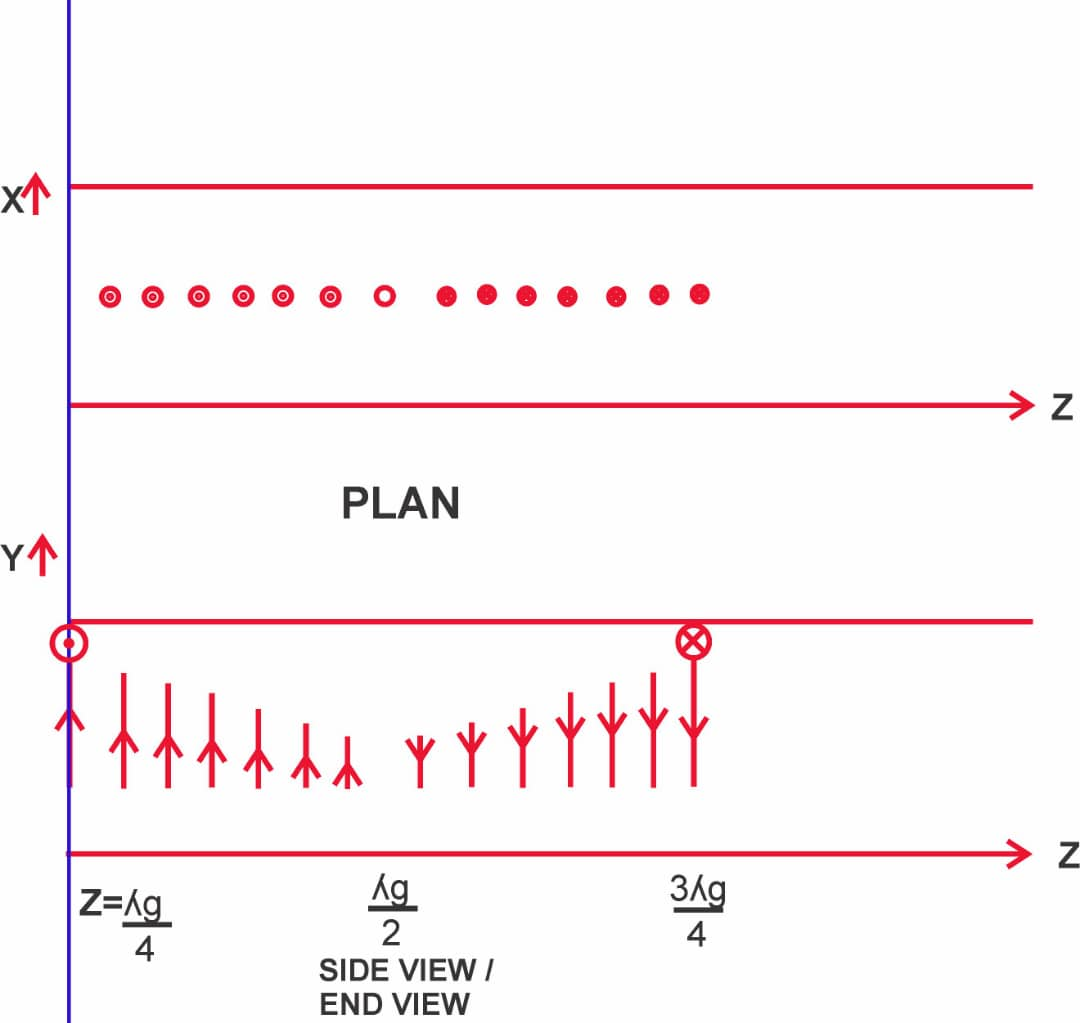
\includegraphics[width=1\linewidth]{./graphics/lecture-image-3.jpg}
\caption{PLAN AND END VIEW OF AN EM WAVE OF A RECTANGULAR WAVE GUIDE}
\end{figure}

As we have seen in the case of parallel plane waveguides, $H_{x}$ have variation same as the electric field by $E_{y}$. $E_{y}$ and $H_{x}$ are maximum at same time and minimum at the same point. But the Z component of magnetic field is shifted by $90^{o}$ or $\frac{\lambda g}{4}$ with respect to the x components. So wherever $H_{x}$ goes to zero, $H_{z}$ is maximum, so it is quadrature in x and z as we see below. We observe that;
\begin{equation}
Re[E_{z}] = C\cos\dfrac{\pi x}{a}\cos\dfrac{2\pi}{\lambda g}z
\end{equation}
\begin{equation}
Re[E_{x}] = B\sin\dfrac{\pi x}{a} \sin\dfrac{2\pi}{\lambda g}z
\end{equation}
So where $H_{x}$ is maximum along Z i.e Z = $\frac{\lambda g}{4}$, $H_{x}$ is minimum.
The magnetic field lines are shown above with arrows designated 1, 2, 3 and 4. Carefully observe $H_{x}$ and $H_{z}$ maximum and where they occur. So because magnetic field must close on itself, 1, 2, 3, 4 must form a loop as shown above.
The variation of the magnetic field in the Y-direction is zero. Hence $H_{x}$ and $H_{z}$ are constant the Y direction. So in the plan view it appears as shown 
\begin{figure}[h]
\centering
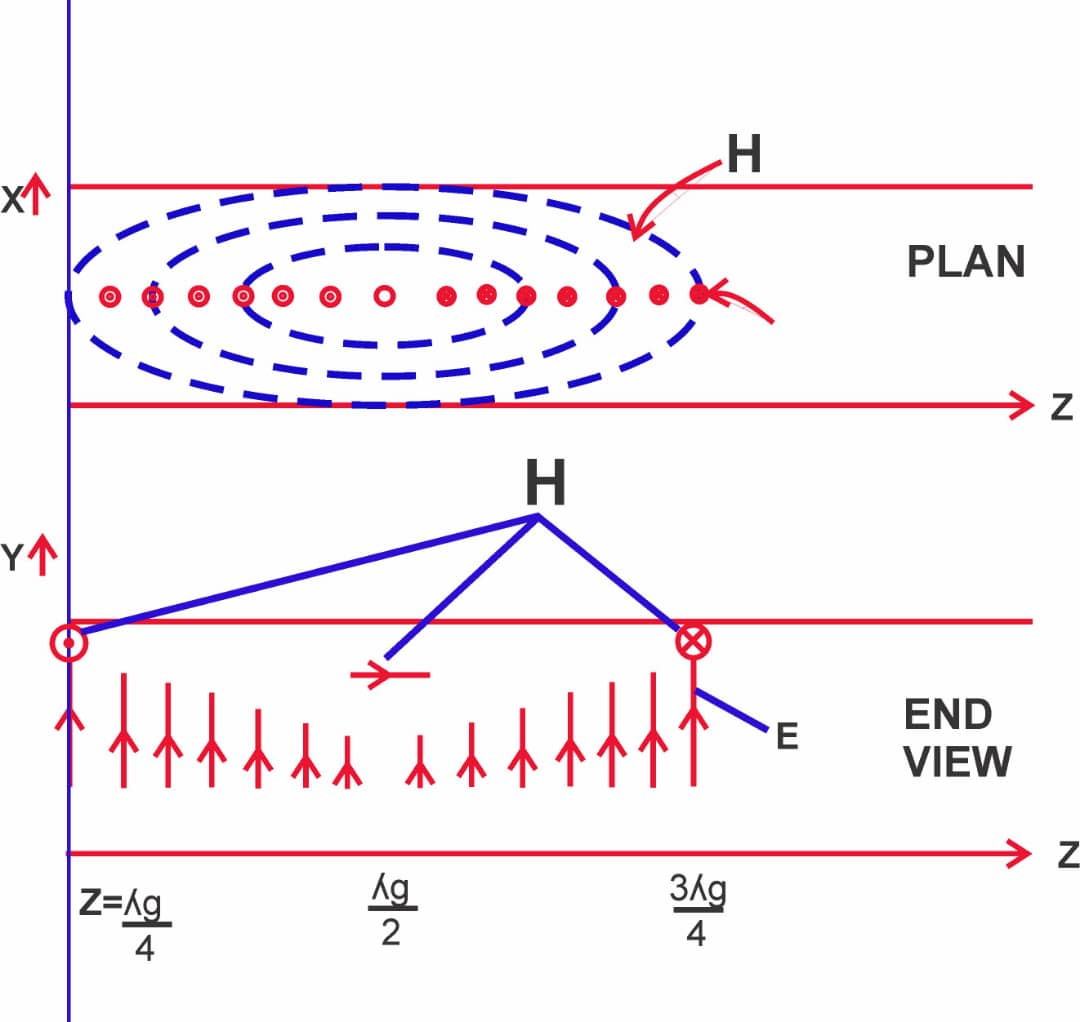
\includegraphics[width=1\linewidth]{./graphics/image-1.jpg}
\caption{PLAN AND END VIEW OF AN EM WAVE OF A RECTANGULAR WAVE GUIDE(SHOWING THE FIELDS)}
\end{figure}

with appropriate direction so that E x H gives the direction of propagation of Z. From the end view, from Z = $\dfrac{\lambda g}{4}$ we have the magnetic field on the side wall coming towards us and at Z = $\dfrac{\lambda g}{2}$ , only $H_{z}$ is represented at 
Z = $\frac{3\lambda g}{4}$. We have $H_{x}$ going in the direction of $\otimes$. So if we visualize this field as a three dimensional structure, the electric fields looks like rods of various various heights or various diameters, where diameters or the heights of the
rod represent the the strength of the electric field and the magnetic field look likes copies of rolled carpets or transformer stampings. shown below is a clever visualization.
\begin{figure}[h]
\centering
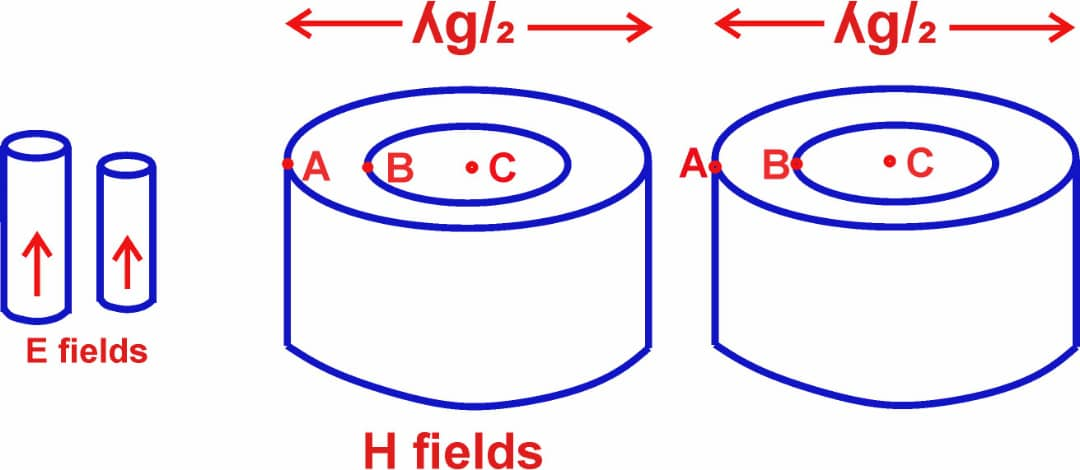
\includegraphics[width=1\linewidth]{./graphics/lecture-image-4.jpg}
\caption{REPRESENTATION OF THE FIELD THREE DIMENSIONAL STRUCTURE}
\end{figure}
	
Now that we get the field visualization at some instant of time, we say let this pattern move with the phase velocity inside the waveguide i.e the pattern starts drifting, so at every location we sometimes see either A,B or C. Now we know that electric field is maximum on the broader wall of the waveguide as mentioned earlier. For the $TE_{10}$ mode, the maximum electric field is along the broad wall along the points   $x = \frac{a}{2}$ as the wave travels in the z direction. The magnetic field would be maximum on wall G and H. It does not vary with Y. So if we have to excite the waveguide by electric fields, with a voltage probe, then the probe must be placed on the line of the broader wall (ie $x = [\dfrac{a}{2}]$ middle point) so that the electric field is excited and that electric field gives excitation corresponding to $TE_{10}$. However, if we have a current probe, we put it on the side walls of G and h which can excite the field distribution shown. Then this would help in exciting $TE_{10}$ Mode inside the waveguide. Same thing is true that if the waveguide was having some modal properties and we want to sense the voltage and current on this waveguide, the voltage probe must be mounted on the broader wall and the current probe must be mounted on the sidewall a and H. This is the way the field inside a rectangular waveguide are detected by using the voltage and current probe, or excited by giving signals to the probe protruding into the waveguides and then excite a field inside a structure.

So this visualization of the field for the dominant mode  which is th the $TE_{10}$ mode is quite useful because it also tells us how the excitation of the field can be achieved by putting voltage and current probes on the wall of the waveguides. Having understood the field distribution in the  $TE_{10}$ mode with electric field more like rod and magnetic field more like rolled carpet or transformer stamping, we can very easily draw the electric and magnetic field for higher order modes. Lets say we want to excite the $TE_{20}$ mode for the rectangular waveguide.

Of course we can write down the field expressions for electric and magnetic fields. Do same thing we did for $TE_{10}$ and visualize the fields. However, once we understood that electric and magnetic field are in specific form, we can stretch our imagination a bit to visualize electric and magnetic field for this higher order mode.

The 2 on $TE_{20}$ mode is telling us that there are two cycles in the X direction and no variation in the Y direction. So the electric field always lie in the Y direction. For the magnetic fields, because the magnetic fields are like stamping or rolled carpets and we are having two sections. Each would have a magnetic loop shown above. The direction of magnetic field will be such that the poynting vector is in the z-direction. In the region between the two magnetic loops, all the fields are essentially going together, so we have two rolled carpets stacked against each others in the waveguide of $TE_{20}$ mode. So once a basic understanding of visualizing fields is developed, it is easy to visualize the fields for higher order modes. The next question we ask is when the fields are excited inside this waveguide, surface current will be induced in the waveguide. Again we come back to $TE_{10}$ mode. We have seen that surface current is related to the tangential component of magnetic fields. So in the figure above, on the top wall, the direction of magnetic field keeps changing, however on the side wall's.The magnetic field direction is always along z direction. Though magnitude is changing, but it is always along the z direction. n x H of side walls, H is in the -y direction i.e going down ward in the y direction
\begin{figure}[h]
\centering
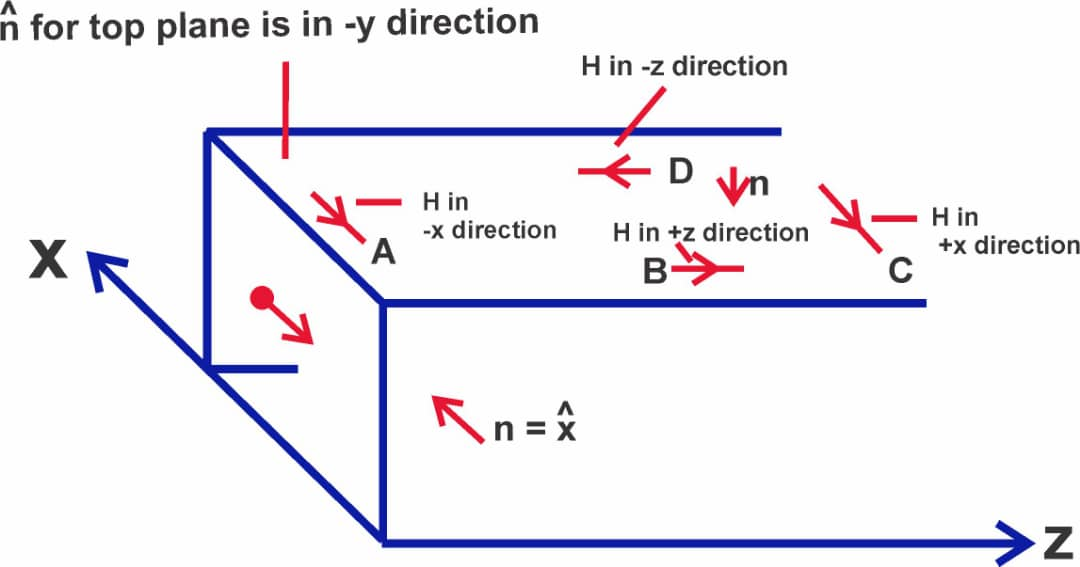
\includegraphics[width=1\linewidth]{./graphics/lecture-image-5.jpg}
\caption{DIRECTION OF THE SURFACE CURRENT AND MAGNETIC FIELD IN A RECTANGULAR WAVEGUIDE}
\end{figure}
\begin{figure}[h]
\centering
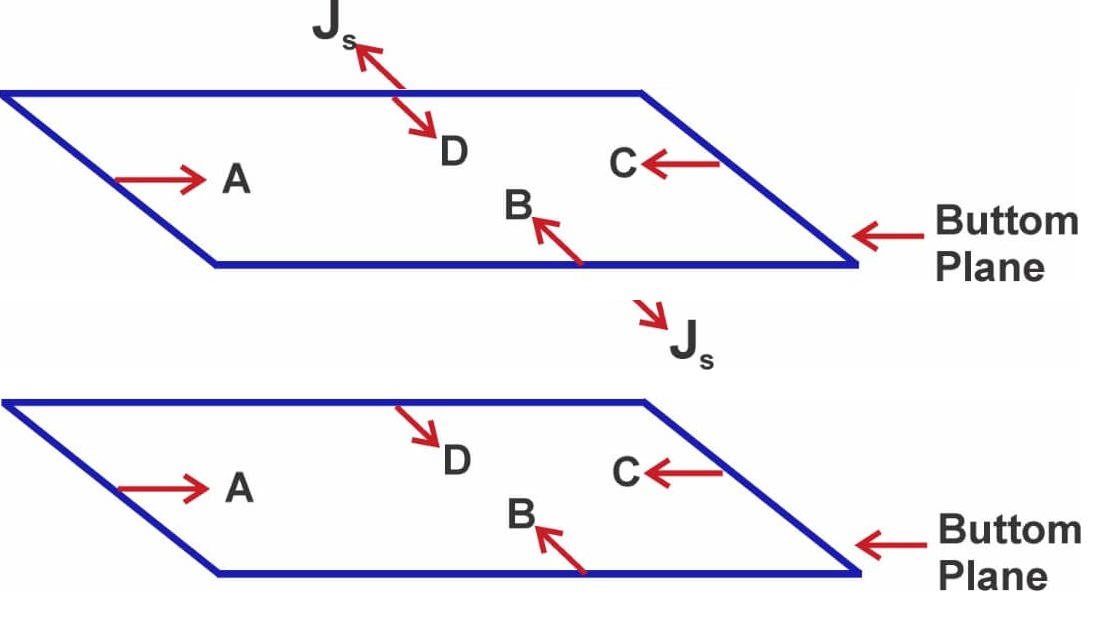
\includegraphics[width=1\linewidth]{./graphics/lecture-image-6.jpg}
\caption{DIRECTION OF THE SURFACE CURRENT AND MAGNETIC FIELD ON THE TOP AND BUTTON PLATE OF A RECTANGULAR WAVE GUIDE}
\end{figure}

On the top plane, At
\begin{equation}
   \hat{n} \times H = -\hat{y} \times (-\hat{x})= -\hat{z}
\end{equation}
\begin{equation}
   \hat{n} \times H = -\hat{y} \times (+\hat{z})= -\hat{x}
\end{equation}
\begin{equation}
    \hat{n} \times H = -\hat{y} \times (+\hat{x})= \hat{z}
\end{equation}
\begin{equation}
    \hat{n} \times H = -\hat{y} \times (-\hat{z})= \hat{z}
\end{equation}
Hence we see the variation of $J_{s}$ as it keeps changing direction in the plane. For right side wall it is in z direction +z and for left side wall it is in -z direction.
Left   
\begin{equation}
n\times H = -\hat{x} \times (-\hat{z})= -\hat{y}
\end{equation}
Right  
\begin{equation}
n \times H = \hat{x} \times (\hat{z}) = \hat{y}
\end{equation}
For the above, the surface current is going in y-direction only upon one face down on the other sign is immaterial here.
	
The bottom plane has the opposite direction for $J_{s}$ corresponding to the top plane as calculated and it is shown above. So looking at the current distribution for all the four walls and combining them together, we have the figure below.
\begin{figure}[h]
\centering
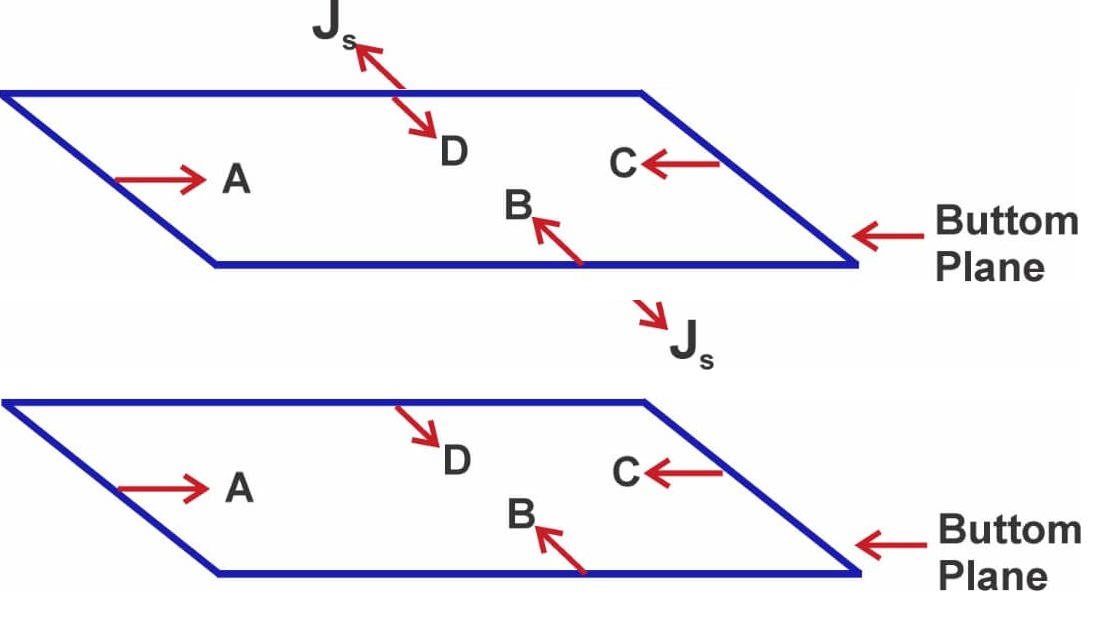
\includegraphics[width=1\linewidth]{./graphics/lecture-image-6.jpg}
\caption{DISTRIBUTION OF CURRENT DENSITY IN A RECTANGULAR WAVE GUIDE}
\end{figure}

So in the figure for the right side wall, the magnetic field was in z-direction and at $\pi$ region $J_{s}$ was in y-direction as we solved above. On the top normal direction is y, so then we have a situation shown where it is as if current is just coming out of the top plane or coming into a point on the top plane or bottom plane depending on the location under consideration. So on the side wall the current does not change as H on the side wall was also constant. It is zero at the center of the top plane, it increases as we get to the side of the top plane, remains constant on the side wall and then decreases till it becomes zero on opposite points to the top wall where H started from. In fact the current is as if it is starting from nowhere it grows and dies down on the opposite to the wall where it started. In the next half cycle, direction of the current will charge and this repeats itself periodically.In one circle the current flows upward that is the charge move downward. In another half cycle, the current flows downward i.e the electrons moves upward. So accumulation of charges takes place between two walls and the charges keep going back and forth and essentially the current flows on the surface of the waveguide. So for every $\frac{\lambda g}{2}$ we have a current island created. It grows and becomes maximum and then decrease to zero on the top plane and bottom plane. It repeats this every $\frac{\lambda g}{2}$. So the current flow is like blooming flower around both sides, with one like a source and other like a sink of current on the opposite top and bottom plane.
	
So this is how the current is going to get induced on the rectangular waveguide. This current helps us to also find out, if we cut the waveguide and allow some slots inside the waveguide, we will see later in antennas that if the current are disrupted, then there is a possibility of getting radiation from the system. So if the current direction in the waveguide is known. them we know where we should cut the slots in the waveguide. So that there is a possibility of radiation. If we cut a slot which does not distort the current flows, as shown in the diagram.

\begin{figure}[h]
\centering
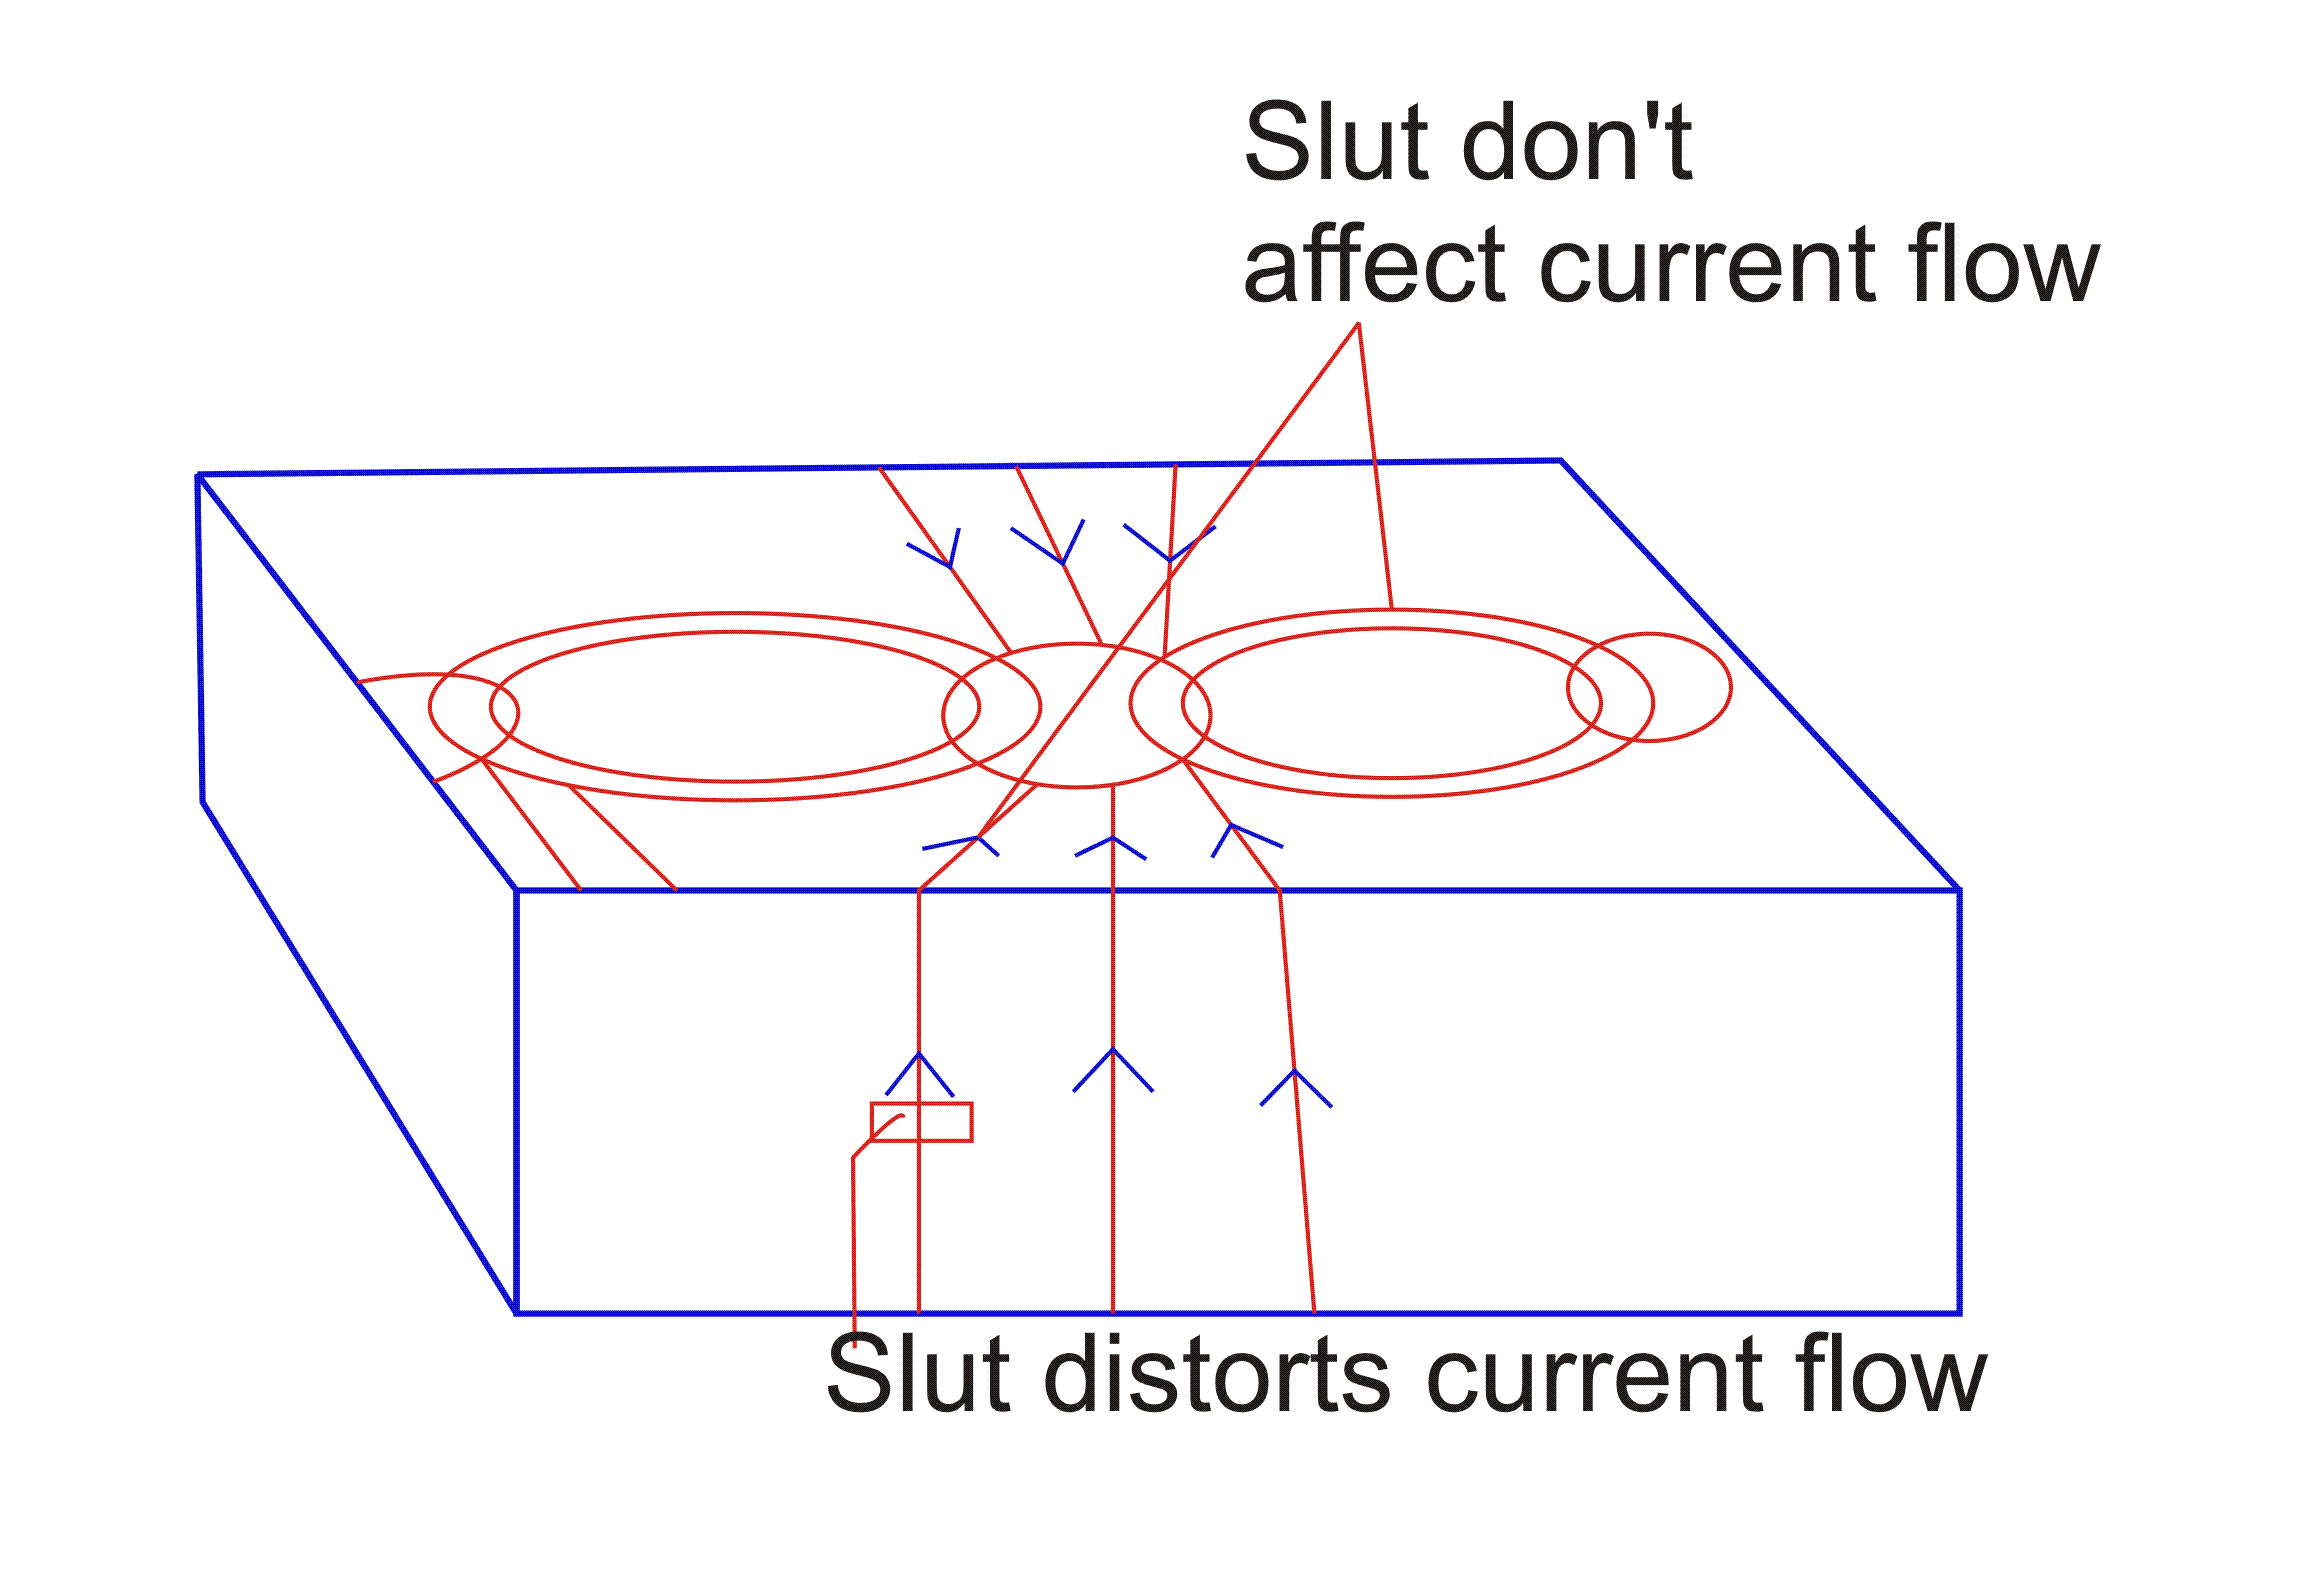
\includegraphics[width=1\linewidth]{./graphics/lecture-image-10.png}
\caption{DIAGRAM SHOWING THE RELATIONSHIP BETWEEN SLOT AND CURRENT FLOW}
\end{figure}
 Because of that there is less possibility of radiation. So if we know the direction of current on this waveguide, we then know were to cut the slots on the waveguide to get radiation.

Another usefulness of finding current direction is if the walls are not ideal conductors, the current flowing will create ohmic losses, that means the power should have been propagated inside the waveguide, part of it will get lost in ohmic heating of the waveguides and this is related to the current distribution on the walls.So the knowledge of current distribution is useful in finding out how the structure can be made to radiate and also how the losses will change if the walls are not ideal conductors.
	
With this, we can go to the next important topic in waveguides i.e the loss calculation in the rectangular waveguide. We have seen that if the structure are not ideal i.e he dielectric filling the the waveguide is not an ideal dielectric, and if the conductor is not ideal conductor, i.e conductivity is not infinite there will always be loss of energy when it propagates through the structure.
Now we try to find out what is the loss per unit length of this waveguide. As we know, it it is measured by a parameter called ATTENUATION CONSTANT.

We have seen in Transmission Line, that if there is a loss in Transmission Line, the variation will be $e^{-\alpha z}$ were $\alpha$ is the attenuation constant. So all the the fields exponentially decays as we travel along the structure. Here we assume that the attenuation constant will cause exponential decay of the fields as they travel. We are interested in finding out the attenuation constant of the conductivity parameter for the walls and the loss in the dielectric is given. However the problem in this case is a little complicated and for this simple reason, if we consider an arbitrary loss in the wall, and arbitrary loss in the dielectric. The modal analysis which we have carried out has to modified now because, the field distribution we earlier assumed we had ideal conductors and ideal dielectric. So in the presence of loss, the electric and magnetic fields are going to get modified, and modification of electric and magnetic fields will change the loss, since the loss is related to current distribution. So essentially we are in a loop that the loss calculation requires the knowledge of electric and  magnetic fields and the electric and magnetic fields depend on the loss.
	
The problems is very complicated, in fact if we went to solve this for arbitrary loss, in the dielectric for arbitrary conductivity of the walls, if assume that the primary function of this waveguide was to transfer energy from one point to the other efficiently, we make every effort to get the losses as minimum as possible.
That means we make a waveguide of a material which has a high conductivity as possible and fill this waveguide with a dielectric as pure as possible. So normally the loss which takes place either in the dielectric filling this waveguide or the finite conductivity of the conducting plane is very very small. Under the assumption, then we can say that as a first order, the fields do not get disturbed significantly because of the losses in the waveguide. What this means is we assume that fields we got for any of the modes are exactly the same as the lossless waveguides even in the presence of this small loss.
So we said that we have a full knowledge of the electric and magnetic fields and once we say that the loop is broken. So from the knowledge of electric and magnetic fields, we can find out what is the current, from there we can find out what is the ohmic losses and then we can calculate attenuation constant. Normally what we will do since attenuation is coming because of the two components viz, loss in the dielectric and then loss in the conducting walls. We separate out these two losses. We say well since the losses are very small, when we calculate dielectric losses, we assume that the waveguide is made of high conductance. When we calculate the conductive losses we assume the waveguide is filled with ideal dielectric. So if we say we have attenuation constant $\alpha$, it consist of two components and two first order approximation, $\alpha$ is the sum of two alphas, $\alpha_{d}$ for dielectric loss and  $\alpha_{c}$ for conductor loss. So $\alpha =  \alpha_{d} +  \alpha_{c}$. When calculating $\alpha_{c}$ we assume  $\alpha_{d} = 0$ and when calculating  $\alpha_{d}$, we assume  $\alpha_{c} = 0$.
	
In calculating  $\alpha_{d}$ we use same approach we used for a Transmission Line. That is we calculate the propagation constant $\beta$ and from the special relation, simply replace the dielectric constant by the dielectric constant of a lossy medium.

\begin{equation}
\beta^{2} = \omega^{2}\mu\epsilon_{l} - (\frac{\pi}{a})^{2}
\end{equation}
for lossy medium. With $\epsilon_{l}$ is for lossy medium, $\beta$ for $TE_{10}$ mode say.
\begin{equation}
\epsilon_{1} = \epsilon_{o}\epsilon_{rl}
\end{equation}
\begin{equation}
\epsilon_{rl} = \epsilon_{r}(1-j\tan\delta)
\end{equation}
Where $\tan\delta$ = loss tangent
We replace $\epsilon_{l}$ by this to have 
\begin{equation}
\beta^{2}_{l} = \omega^{2}\mu\epsilon_{o}\epsilon_{r}(1-j\tan\delta)
\end{equation}
$\tan\delta$ is usually small for low loss dielectric medium.
$$
\beta^{2}_{l} = \omega^{2}\mu\epsilon_{o}\epsilon_{r} - j\omega^{2}\mu\epsilon_{o}\epsilon_{r}\tan\delta$$
$$ = \beta^{2} - j\beta^{2}\tan\delta \equiv \beta^{2} - j\omega^{2}\epsilon_{o}\epsilon_{r}\tan\delta
$$
\begin{align}
\beta_{l} = (\beta^{2} - j\omega\mu\epsilon_{o}\epsilon_{r}\tan\delta)^{\frac{1}{2}} \simeq \beta - \dfrac{j\omega^{2}\mu\epsilon_{o}\epsilon_{r}\tan\delta}{2\beta}
\end{align}
So we have a phase constant $\beta_{l}$ which as a real and imaginary part. The real part is $\beta$. Attenuation constant due to lossy dielectric filling the waveguide
\begin{align}
 \alpha_{d} = \dfrac{\omega^{2}\mu\epsilon_{o}\epsilon_{r}\tan\delta}{2\beta}
\end{align}
Recall in waveguide the variation along z is $e^{-j\beta z}$ so you need imaginary values of $\beta$ to give you attenuation. A real value would give oscillatory terms in $\cos\beta z$ and $\sin\beta z$. $e^{-j}(\dfrac{j\omega^{2} \mu\epsilon_{o}\epsilon_{r}\tan\delta}{2\beta})$
becomes an exponentially decaying term.

Since we know that $\tan\delta = \dfrac{\sigma}{\omega\epsilon_{o}\epsilon_{r}}$, We substitute into $$\alpha_{d} = \dfrac{\omega^{2}\mu\epsilon_{o}\epsilon_{r}\tan\delta}{2\beta}$$ to have 
$$
	\alpha_{d} = \dfrac{\omega^{2}\mu\epsilon_{o}\epsilon_{r}\frac{\sigma}{\omega\epsilon_{o}\epsilon_{r}}}{2\beta} = \dfrac{\omega\mu\sigma}{2\beta}
$$
Given the expression for $\beta$ for the lossless case, for the $TE_{10}$ mode which was related to the cutoff frequency of the mode, 
$$
\alpha_{d} =  \frac{\sigma\eta}{2\sqrt{1-(\frac{fc}{f})^{2}}}
$$
where $\eta$ is the intrinsic impedance in the dielectric.
$$	
\eta =  \sqrt{\frac{\mu_{o}}{\epsilon_{o}\epsilon_{r}}}
$$
For lossless case, 
$$\beta = \sqrt{\omega^{2}\mu\epsilon-(\dfrac{m\pi}{a})^{2}-(\dfrac{n\pi}{b})^{2}}$$
For $TE_{10}$ we had, $$\omega^{2}_{c}\mu\epsilon = (\dfrac{m\pi}{a})^{2}+(\dfrac{n\pi}{b})^{2}$$	
As such $$\beta = \sqrt{\omega^{2}\mu\epsilon-\omega^{2}_{c}\mu\epsilon} = \omega\sqrt{\mu\epsilon}\sqrt{1-(\dfrac{fc}{f})^{2}}$$,	
$$\alpha_{d}=\dfrac{\omega\mu\sigma}{2\beta}= \dfrac{\omega\mu\sigma}{2\omega\sqrt{\mu\epsilon}\sqrt{1-(\dfrac{fc}{f})^{2}}}$$\\
Divide numerator by $\omega\sqrt{\mu\epsilon}$
$$= \dfrac{\sigma\sqrt{\frac{\mu}{\epsilon}}}{2\sqrt{1-(\dfrac{fc}{f})^{2}}}$$\\
$=\dfrac{\sigma\eta}{2\sqrt{1 - (\dfrac{fc}{f})^{2}}}$ where $\eta= \sqrt{\frac{\mu}{\epsilon}}$\\
Therefore $\alpha_{d} = \dfrac{\sigma\eta}{2\sqrt{1 -(\frac{fc}{f})^{2}}}$ and $f_c$ is the cut-off frequency of the mode under consideration.

So knowing the dielectric constant of the medium and assuming the loss tangent is very small, ie the losses in the medium are very small, we can establish the attenuation constant $\alpha_{d}$ due to the finite conductivity of the dielectric medium. We say that for two losses, the attenuation constant is proportional to the conductivity of the medium and we see that $\alpha_{d}$ is related t cut-off frequency.
So when frequency is much larger compared to $f_{c}$, we have $\dfrac{\sigma\eta}{2}$ which is very similar to the case of Transmission Line. We recall that if we take the transverse electromagnetic mode, $\frac{\sigma}{2}(\eta)$ was the attenuation constant for the Transmission Line.
So when we talk about the lossy mediums in the unbound medium, that time we get a loss which was $\alpha = \dfrac{\sigma\eta}{2}$. What happens now however is that in the rectangular waveguide, it also depends upon how far away you are from the cut-off frequency, so if you are very close to cut-off frequency, $\sqrt{1 - (\dfrac{fc}{f})^{2}}$ becomes close to zero.
$\dfrac{\sigma\eta}{2\sqrt{1-(\dfrac{fc}{f})^{2}}}$ becomes very large and the dielectric loss $\alpha_{d}$ becomes very large. So now the dielectric loss is a function of frequency which otherwise was not a function of frequency. In the transverse electromagnetic mode,  $\alpha_{d}$ only depended on the conductivity. So $\alpha_{d}$ is proportional to the conductivity of the dielectric $\sigma$, It also depends on how far away you are from the cut-off frequency of a particular mode. As you go closer to the cut-off frequency of a particular mode. As you go closer to the cut-off frequency of the mode, your dielectric loss increases. So by using this we can calculate one component of the attenuation constant and that is the dielectric attenuation constant $\alpha_{d}$.

The second component we want to calculate now is due to finite conductivity of the boundary. this calculation is not as straightforward as this we have just done. Since fields are now inside the waveguide. Simply modifying the propagation constant, but we do not know now how to put this medium as a lossy medium. If the losses are going to take place in the walls. So what we have to do is to go from the first principle and calculate the attenuation constant using first principles. What this means is that if there is a loss in the medium, the $E$ and $H$ of the fields vary as a function of $z$ ie $ {\hat{E}}, {\hat{H}} \ \sim\ e^{-\alpha z}$ where $\alpha$ is the attenuation constant. So the power which is proportional to $|{\hat{E}}|^{2}$ or $|{\hat{H}}|^{2}$ since power is ${\hat{E}}\times={\hat{H}}$. So power density is the power which the waveguide carriers, i.e $\omega\sim e^{-2\alpha z}$ ie varies as $e^{-2\alpha z}$. We can differentiate $\omega$ power with respect to z to get $$\dfrac{dw}{dz}\sim-2\alpha e^{-2\alpha z} = -2\alpha\omega$$ So that $\alpha$ the attenuation constant in general. If we calculate $$\alpha = \dfrac{-\frac{dw}{dz}}{2w}$$ $$w = -2\exp^{-2\alpha z}$$ $$\frac{dw}{dz} = -2\omega_{o} e^{-2\alpha z} = -2\alpha w$$. $$\alpha = \dfrac{-\frac{dw}{dz}}{2w}$$ Physically -$\frac{dw}{dz}$ stands for the rate at which power decrease in the direction $z$ or in the direction of the wave propagation. W is the total power carried by the structure. Now that the attenuation constant can be calculated by two quantities i.e power loss per unit length $(-\dfrac{dw}{dz})$  along the waveguide, divided by two times the power carried by the waveguide.

$\alpha = \dfrac{\textnormal{power decrease / unit length}}{2\times \textnormal{Total power carried by the waveguide}}$
\paragraph{Calculating for attenuating constant:}
Now to calculate the attenuation constant, we require two quantities to be calculated viz power loss per unit length and the total power carried by the waveguide. So if we go to the rectangular waveguide, we have to calculate two things. These is E and H for the waveguide and surface current that will flow in all the four walls. So surface current will give us the loss, and we can calculate it per unit length i.e what is the power loss in the waveguide. Calculating $E\times H$ will give the poynting vector and integrating over the cross sectional  area of the waveguide gives the total power flowing inside the waveguide. So $w = \int\frac{Re}{2}(\bar{E}\times\bar{H^*})={da} = \int \frac{1}{2}Re(\bar{E}\times {H}^*).{da}$ gives the total power flowing in  the waveguide. Once we know the surface current $I_{s}$ on these walls, then we see that power loss per unit area is given by half surface resistance multiplied by $|J_{s}|^{2}$. So knowing the surface current, we can calculate the loss per unit area and since the height of the waveguide is known, we can calculate the loss per unit length of the waveguide. Once we know these two quantities, using the relation $\alpha = -\dfrac{\frac{dw}{dz}}{2w}$, we can calculate the attenuation constant of this waveguide due to finite conductivity of the walls.

In the next lecture, by using the basic definition of the attenuation constant, we will derive the attenuation constant for two modes. One is for a parallel plane waveguide in the TEM mode, i.e the simplest mode just to get a feel of how to calculate this quantity. Then we would go to the calculation of the attenuation constant for a rectangular waveguide for $TE_{10}$ mode. 